\subsection{\label{sub:\projectname-Calculadora} \textsf{Calculadora}}

\paragraph{Símbol}

\begin{center} \bsfsymbol{Calculadora} \end{center}

\paragraph{Entrades i sortides}

\begin{where}
\item[\nodenamebit{sigA}] Signe del primer factor
\item[\nodenamerange{A}{3}{0}] Mòdul del primer factor (BCD)
\item[\nodenamebit{sigB}] Signe del segon factor
\item[\nodenamerange{B}{3}{0}] Mòdul del segon factor (BCD)
\item[\nodenamebit{sigRes}] Signe del producte
\item[\nodenamerange{res}{7}{0}] Mòdul del producte (BCD)
\item[\nodenamerange{selop}{1}{0}] Índex d'operació a realitzar
\end{where}

\paragraph{Funció}

Calculadora BCD d'una xifra amb signe, amb resultat en dues xifres.

Retorna a les sortides $sigRes$ i $res$ el signe i mòdul de la operació corresponent,
segons el valor de $selop$:

\begin{description}
\item[00] Producte de $A$ per $B$
\item[01] Quadrat de $A$
\item[10] Quadrat de $B$
\item[11] Suma de $A$ amb $B$
\end{description}

\paragraph{Inespecificacions}


La sortida no està definida si $A$ o $B$ no pertanyen al seu codi.


\paragraph{Implementació}

\vhdlisting{Calculadora}



Per a les primeres tres operacions ($selop \neq 11$), el resultat s'agafa d'un
bloc \textsf{AperB} amb les dues entrades com sigui oportú. Per a l'última operació,
la sortida prové d'un bloc \textsf{AmesB}.

\paragraph{Simulació}

\begin{contendfig}
  \begin{center}
    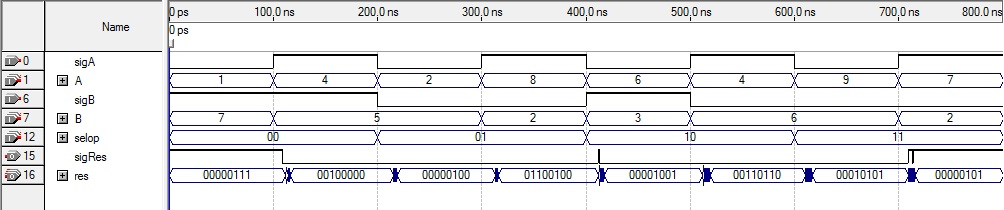
\includegraphics[scale=0.55]{../\projectname/assets/vwf/Calculadora.jpg}
  \end{center}
  \caption{\label{fig:sim-\projectname-Calculadora} Simulació per al bloc \textsf{Calculadora}}
\end{contendfig}

La simulació del bloc es pot veure a la figura~\ref{fig:sim-\projectname-Calculadora} (pàgina~\pageref{fig:sim-\projectname-Calculadora}).

% FIXME

\vspace{1cm}
